\section{Proposed Methodology}
\label{sec:method}

This section specifies the framework in full: the data, the exact form of every input
feature, the regime model, the fusion rule, the optimisation problem, and the
walk-forward protocol under which it is evaluated. The level of detail is deliberate,
so that the study can be reproduced independently from this description alone.

\begin{figure*}[t]
\centering
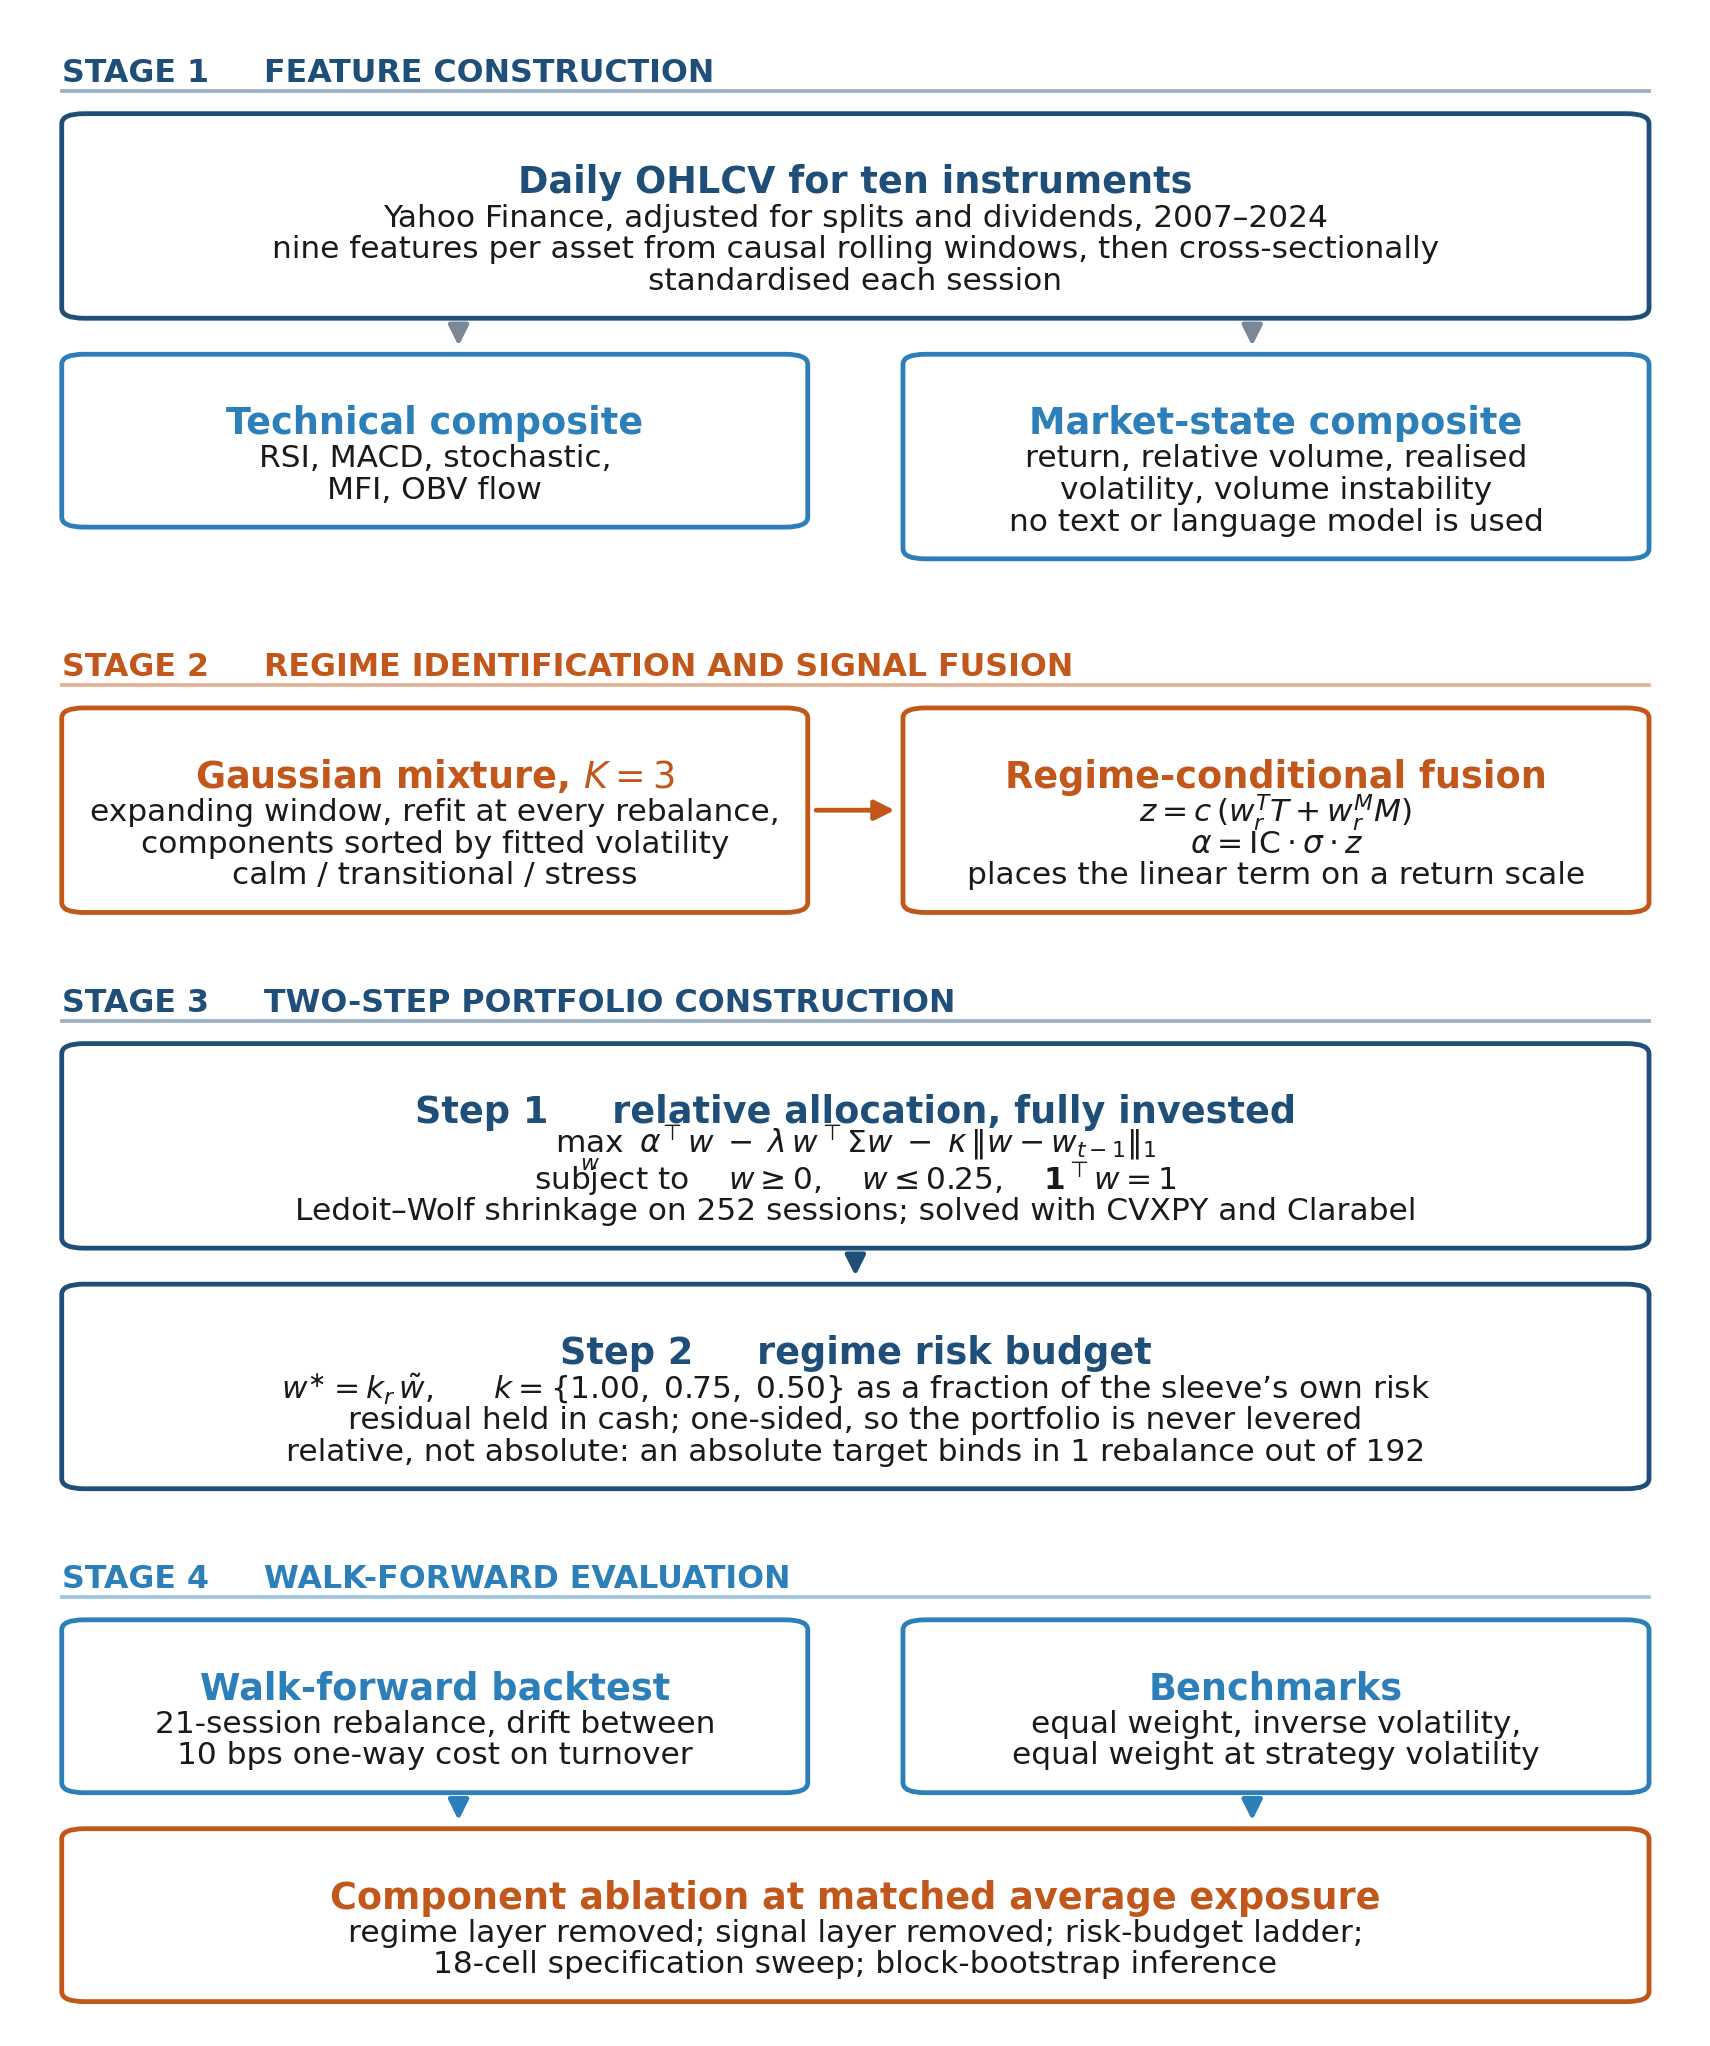
\includegraphics[width=\textwidth]{single column/images/fig_architecture.png}
\caption{The proposed framework. Stage~1 constructs causal, cross-sectionally
standardised features; stage~2 identifies the market state and fuses the two composites;
stage~3 separates relative composition from total risk; stage~4 evaluates the result and
ablates its components.}
\label{fig:architecture}
\end{figure*}

\subsection{Data and Study Universe}

The primary study universe consists of ten exchange-traded funds selected to span the
major liquid asset classes available to a diversified allocator: US large capitalisation
equity (SPY), US large capitalisation growth equity (QQQ), US small capitalisation
equity (IWM), developed international equity (EFA), emerging market equity (EEM),
long-maturity US Treasuries (TLT), intermediate-maturity US Treasuries (IEF),
investment-grade corporate credit (LQD), gold (GLD) and US real estate (VNQ). Breadth
matters for the research question. A framework whose stated purpose is to redirect risk
across market states can only be tested where there is somewhere else for risk to go;
a single-sector universe offers no such destination, a point returned to in
Section~\ref{sec:megacap}.

Daily open, high, low, close and volume series are obtained from Yahoo Finance through
the \texttt{yfinance} interface, adjusted for splits and dividends. The download window
is 1~January 2007 to 27~August 2026. The end date is not a modelling choice: it is
every session available at the date the analysis was run, so the sample boundary
carries no information about the results. Indicator warm-up and the 252-session covariance
estimation window consume the first year, so the evaluated out-of-sample period runs
from January 2008 to August 2026 and covers the global financial crisis, the 2011
sovereign debt episode, the 2020 pandemic crash, the 2022 inflation-driven bear market
and the subsequent recovery.

Sessions from 1~January 2024 onward are treated as a holdout. That block postdates
the design of the framework and every specification decision reported here; none of
it was examined while the model was being built. It enters the full-sample results
for completeness and is reported separately in Section~\ref{sec:holdout}, where it
serves as an out-of-sample check rather than as evidence used in fitting. A secondary
universe of ten mega-capitalisation US equities over 2018--2026 is carried through the
same pipeline and reported separately in Section~\ref{sec:megacap}.

\subsection{Feature Construction}

Nine features are computed for each asset on each session. All are causal: every value
at session $t$ uses only information available at the close of session $t$. Table~\ref{tab:features}
gives the exact definition of each, and no other input enters the framework.

\begin{table}[!ht]
\centering
\caption{Input features. $C_t$, $H_t$, $L_t$ and $V_t$ denote close, high, low and
volume. All features are computed per asset, then cross-sectionally standardised.}
\label{tab:features}
\small
\begin{tabular}{p{2.0cm}p{1.8cm}p{5.2cm}p{1.5cm}}
\hline
\textbf{Feature} & \textbf{Composite} & \textbf{Definition} & \textbf{Window} \\
\hline
RSI & Technical & Relative strength index, centred: $\mathrm{RSI}_t - 50$ & 14 \\
\hline
MACD & Technical & Moving average convergence divergence line, scaled by price: $\mathrm{MACD}_t / C_t$ & 12, 26, 9 \\
\hline
Stochastic & Technical & Stochastic oscillator \%K, centred: $\%K_t - 50$ & 14, smooth 3 \\
\hline
MFI & Technical & Money flow index, centred: $\mathrm{MFI}_t - 50$ & 14 \\
\hline
OBV flow & Technical & Twenty-session change in on-balance volume, normalised by average volume: $(\mathrm{OBV}_t - \mathrm{OBV}_{t-20}) / \overline{V}_{t,20}$ & 20 \\
\hline
Return & Market state & Five-session simple return: $C_t / C_{t-5} - 1$ & 5 \\
\hline
Relative volume & Market state & $V_t / \overline{V}_{t,20}$ & 20 \\
\hline
Realised volatility & Market state & Annualised standard deviation of daily returns, entered with a negative sign & 20 \\
\hline
Volume instability & Market state & Standard deviation of daily volume changes, entered with a negative sign & 20 \\
\hline
\end{tabular}
\end{table}

Each feature is standardised cross-sectionally on every session, so that a value
expresses how an asset ranks against its peers that day rather than against its own
history. Writing $x_{i,t}$ for the raw feature of asset $i$ and $N$ for the number of
assets,
\begin{equation}
z_{i,t} = \frac{x_{i,t} - \bar{x}_t}{s_t}, \qquad
\bar{x}_t = \frac{1}{N}\sum_{j} x_{j,t}, \qquad
s_t = \mathrm{sd}_j(x_{j,t}).
\end{equation}
Cross-sectional standardisation is used rather than time-series standardisation because
the allocation problem is a relative one: the optimiser must decide which assets to
prefer today, not whether today is unusual by historical standards. It also removes the
common market factor from the scores, so that a market-wide move does not appear as a
signal on every asset simultaneously.

The standardised features are then averaged into two composites. The technical
composite is the equally weighted mean of the five technical features. The market-state
composite is the equally weighted mean of the four market-state features, taken with
the signs given in Table~\ref{tab:features}, so that recent strength and active participation raise the
score while realised volatility and unstable volume lower it.

\subsection{What the Second Composite Is, and What It Is Not}
\label{sec:notsentiment}

The second composite is constructed entirely from price and volume. No news article,
social media post, corporate announcement or any other text is read at any point in
this study, and no lexicon, classifier or language model is applied. The composite is a
market-derived proxy for the same latent quantities that textual sentiment measures aim
to capture---attention, participation and stress---and it is reported here as exactly
that.

This is stated plainly because the distinction is material to how the results should be
read. Proxy construction of this kind is common in the literature and inexpensive to
compute, but it cannot be credited with the contextual information a transformer model
extracts from financial text, and it should not be described as though it could.
Section~\ref{sec:ic} measures the predictive content of both composites directly and
reports the outcome, including where that outcome is unfavourable. Extending the
framework to genuine textual sentiment requires a time-stamped news corpus with
coverage of the traded universe; for broad exchange-traded funds no such corpus exists
at instrument level, which is a limitation of the design rather than an oversight, and
Section~5 sets out what would be needed to remove it.

\subsection{Regime Identification}

Market states are identified with a Gaussian mixture model over two features, each
computed as a cross-sectional average across the universe: the twenty-session rolling
standard deviation of daily returns, and the ten-session rolling mean of daily returns.
The first captures the volatility of the environment, the second its direction. Both
are standardised before fitting.

The mixture uses $K = 3$ components with full covariance matrices, three random
restarts and a fixed seed. It is refitted at every rebalance date on an expanding
window containing only sessions strictly earlier than that date, with a minimum of 252
observations; the state of the current session is then obtained by prediction from that
fit. No observation ever contributes to the model that labels it.

One implementation detail is essential and is easy to overlook. The component indices
returned by a mixture fit are arbitrary and permute freely between refits, so labels
from consecutive fits are not comparable unless they are anchored. Components are
therefore sorted in ascending order of fitted mean volatility before use, which makes
regime~0 the calm state, regime~1 the transitional state and regime~2 the stress state
consistently across every refit. Omitting this step does not produce an error; it
produces a silently scrambled regime series and, if the resulting labels are compared
across fits, a spurious appearance of instability.

The choice $K = 3$ is not selected by information criterion. As
Section~\ref{sec:regimefit} reports, both the Akaike information criterion (AIC)
and the Bayesian information criterion (BIC) continue to fall as components are added
over the range tested, which is the usual behaviour of mixture models on
persistent financial series and reflects their tendency to absorb heavy tails with
additional components. The choice is instead made on persistence and interpretability:
three components yield states that last long enough to act on and that admit a clear
economic reading, whereas finer partitions fragment into short-lived states that a
monthly rebalancing schedule cannot exploit. This is a modelling judgement and is
reported as such.

\subsection{Regime-Conditional Signal Fusion}

The two composites are combined into a single score using weights that depend on the
prevailing regime, together with a per-asset confidence term. Let $T_{i,t}$ and
$M_{i,t}$ denote the standardised technical and market-state composites for asset $i$,
and let $r_t \in \{0,1,2\}$ be the regime. The fused score is
\begin{equation}
z_{i,t} = c_{i,t} \left[ w^{T}_{r_t} T_{i,t} + w^{M}_{r_t} M_{i,t} \right],
\end{equation}
with regime weights $(w^T, w^M)$ of $(0.7, 0.3)$ in the calm state, $(0.5, 0.5)$ in the
transitional state and $(0.3, 0.7)$ in the stress state. The direction of this schedule
follows the hypothesis stated in Section~1, that trend-following information is more
reliable in quiet trending markets while attention and stress information becomes
relatively more informative when markets are disturbed. Section~\ref{sec:ic} tests that
hypothesis rather than assuming it.

The confidence term $c_{i,t}$ down-weights assets whose two composites disagree:
\begin{equation}
c_{i,t} = \mathrm{clip}\!\left(0.5 + 0.5\,\rho^{(63)}_{i,t}, \; 0.1, \; 1.0\right),
\end{equation}
where $\rho^{(63)}_{i,t}$ is the trailing 63-session correlation between the two
composites for that asset. Agreement between independent views is treated as evidence;
disagreement is treated as noise and shrinks the score toward zero.

The fused score is converted into an expected excess return using the standard
information-ratio scaling of \citet{grinold00}, which places the score on a return
scale rather than leaving it as a dimensionless quantity:
\begin{equation}
\alpha_{i,t} = \mathrm{IC} \cdot \sigma_{i,t} \cdot z_{i,t},
\label{eq:alpha}
\end{equation}
where $\sigma_{i,t}$ is the annualised volatility of asset $i$ from the current
covariance estimate and $\mathrm{IC} = 0.05$ is an assumed information coefficient (IC).

Equation~(\ref{eq:alpha}) is not a cosmetic step. If a raw indicator is passed to a
mean-variance objective directly, the units of the linear term and of the quadratic
risk term are unrelated, and their ratio---not the information in the signal---decides
the solution. An indicator such as on-balance volume takes values of order $10^{8}$ to
$10^{9}$, whereas annualised variances are of order $10^{-2}$; the linear term then
dominates by ten orders of magnitude and the optimiser degenerates to a corner
solution, holding a single asset regardless of the risk model. Section~\ref{sec:alloc}
documents this failure mode explicitly, because it is the source of a behaviour visible
in the originally submitted results.

\subsection{Portfolio Construction}

Allocation proceeds in two steps, which separate two decisions that are often conflated:
which assets to hold relative to one another, and how much total risk to carry.

\paragraph{Step 1: relative allocation.} The risky sleeve solves a quadratic program
with a linear transaction-cost penalty,
\begin{align}
\max_{w} \quad & \alpha_t^{\top} w - \lambda \, w^{\top} \Sigma_t w
- \kappa \left\| w - w_{t-1} \right\|_1 \\
\text{s.t.} \quad & w \geq 0, \qquad w \leq w_{\max}, \qquad \mathbf{1}^{\top} w = 1,
\end{align}
where $\Sigma_t$ is the annualised covariance matrix, $\lambda = 2$ is the risk
aversion coefficient, $w_{\max} = 0.25$ caps any single position at one quarter of the
sleeve, and $w_{t-1}$ is the weight vector carried in from the previous rebalance. The
turnover penalty $\kappa = c \cdot 252 / h$ annualises a one-way cost of $c = 10$ basis
points over a rebalancing interval of $h = 21$ sessions, so that the cost of trading is
expressed on the same annual basis as the return and risk terms.

The equality constraint $\mathbf{1}^{\top} w = 1$ is what makes this step purely
relative. It fixes the sleeve to be fully invested, so the optimiser can only express a
view about composition, never about how much risk to take. That second decision is made
explicitly in step~2 instead of emerging as a by-product of the constraint set.

$\Sigma_t$ is estimated by Ledoit--Wolf shrinkage \citep{ledoit04} on the trailing 252
daily returns and annualised by a factor of 252. Shrinkage is used because a sample
covariance matrix estimated from 252 observations on ten assets is poorly conditioned,
and a mean-variance optimiser will concentrate weight precisely on the directions in
which the estimate is least reliable. The problem is convex and is solved with CVXPY
using the Clarabel interior-point solver.

\paragraph{Step 2: regime risk budget.} The sleeve is then scaled by a factor that
depends only on the regime:
\begin{equation}
w^{\ast}_t = k_{r_t} \, \tilde{w}_t, \qquad
k = \{\,\text{calm}: 1.00, \;\; \text{transitional}: 0.75, \;\; \text{stress}: 0.50\,\},
\label{eq:budget}
\end{equation}
with the residual $1 - k_{r_t}$ held in cash, which is assumed to earn zero. Scaling is
one-sided: the framework de-risks in disturbed states but never levers up in calm ones,
so any performance difference is attributable to risk reduction rather than to leverage.

The budget in Equation~(\ref{eq:budget}) is expressed as a fraction of the sleeve's own
risk rather than as an absolute volatility target, and this choice is consequential.
An absolute target de-risks only when the sleeve's estimated volatility exceeds the
target level, so its effect depends on the volatility of the universe it is applied to.
Targets calibrated for a concentrated equity portfolio---of the order of 10 to 20 per
cent annualised---are simply never reached by a diversified ten-asset sleeve whose own
realised volatility is close to 7~per~cent. Under those targets the constraint binds in
one rebalance out of 224 in this study, and the regime layer is inert: it is present in
the specification, consumes computation, and does nothing. A relative budget is
scale-free by construction and remains active in any universe.
Section~\ref{sec:ablation} reports both variants and the difference between them.

\subsection{Walk-Forward Protocol}

The framework is rebalanced every 21 sessions. Between rebalances positions are held
and allowed to drift with realised returns, so that reported turnover reflects trading
actually undertaken rather than a notional daily reweighting. One-way transaction costs
of 10 basis points are charged on the traded fraction $\|w^{\ast}_t - w_{t-1}\|_1$ on
the rebalance session; Section~\ref{sec:cost} varies this assumption from 0 to 25 basis
points.

Every estimated quantity uses only data preceding the decision it informs: the
covariance matrix from the trailing 252 sessions before the rebalance date, the mixture
model from an expanding window strictly earlier than that date, and all features from
causal rolling windows. No parameter is tuned on the evaluation period; the
configuration reported as primary is the one specified above, and
Section~\ref{sec:robust} reports the full grid of alternatives rather than the best
cell of it.

\subsection{Evaluation Design}

Performance is summarised by compound annual growth rate (CAGR), annualised
volatility, Sharpe ratio computed at a zero risk-free rate, maximum drawdown (Max DD)
and Calmar ratio. Three
benchmarks are used. The first is an equal-weighted portfolio of the same ten assets,
rebalanced daily and charged no transaction costs, which is deliberately a generous
comparator. The second is an inverse-volatility portfolio using trailing 60-session
standard deviations, also costless, which isolates whether the framework adds anything
beyond elementary risk weighting. The third rescales the equal-weighted portfolio to
the strategy's realised volatility, which removes the mechanical advantage a
lower-risk portfolio enjoys in ratio comparisons.

Statistical inference on daily excess returns uses a paired $t$-test, a Newey--West
$t$-statistic with ten lags to accommodate autocorrelation and heteroskedasticity, and
a stationary block bootstrap with 21-session blocks and 2{,}000 replications for
interval estimates of the Sharpe ratio and of the Sharpe difference. Component
contributions are isolated by ablation: removing the regime layer while holding average
exposure fixed, removing it while holding full exposure, and removing the signal layer
entirely. Robustness is assessed over a grid of random seeds, covariance estimation
windows and rebalancing frequencies, with every cell reported.
